% MS1 project proposal. Build with ./docs/build.sh proposal (xelatex).
% Hard limit: 2 pages. build.sh warns if the PDF grows past that.
\documentclass[10pt,a4paper]{article}

% xelatex + OpenType so en dashes, curly quotes and "~" render correctly.
\usepackage{fontspec}
\setmainfont{lmroman10-regular.otf}[
  BoldFont       = lmroman10-bold.otf,
  ItalicFont     = lmroman10-italic.otf,
  BoldItalicFont = lmroman10-bolditalic.otf]
\setmonofont{lmmono10-regular.otf}[Scale=MatchLowercase]

\usepackage[a4paper,margin=1.5cm,headsep=4mm]{geometry}
\usepackage{graphicx}
\usepackage{booktabs}
\usepackage{tabularx}
\usepackage{amsmath}
\usepackage{xcolor}
\usepackage{microtype}
\usepackage{caption}
\usepackage{enumitem}
\usepackage{titlesec}
\usepackage{fancyhdr}
\usepackage{tikz}
\usetikzlibrary{positioning,shapes.geometric,arrows.meta,calc}
\usepackage[hidelinks]{hyperref}

\definecolor{hslu}{HTML}{1F4E79}
\definecolor{pipefill}{HTML}{D6E4F7}\definecolor{pipeline}{HTML}{2F5F9E}
\definecolor{storefill}{HTML}{FDEBD3}\definecolor{storeline}{HTML}{B5702F}
\definecolor{outfill}{HTML}{DCEDC8}\definecolor{outline}{HTML}{4A7C3F}
\definecolor{srcfill}{HTML}{EDEDED}

\tikzset{
  box/.style   = {draw, rounded corners=2pt, align=center, font=\scriptsize,
                  minimum width=3.0cm, minimum height=1.05cm, inner sep=2pt},
  pipe/.style  = {box, fill=pipefill, draw=pipeline, line width=0.9pt},
  src/.style   = {box, fill=srcfill, draw=black!60},
  sink/.style   = {box, fill=outfill, draw=outline},
  store/.style = {cylinder, shape border rotate=90, aspect=0.18, draw=storeline,
                  fill=storefill, align=center, font=\scriptsize,
                  minimum width=3.0cm, minimum height=1.15cm, inner sep=1pt},
  flow/.style  = {-{Stealth[length=2mm]}, line width=0.7pt, draw=black!75},
  lbl/.style   = {font=\tiny, fill=white, inner sep=1pt, align=center},
}

\titleformat{\section}{\normalfont\large\bfseries\color{hslu}}{\thesection}{0.6em}{}
\titlespacing*{\section}{0pt}{1.0ex plus .2ex}{0.45ex}
\setlength{\parindent}{0pt}
\setlength{\parskip}{0.42ex plus 0.2ex minus 0.1ex}
\captionsetup{font=small,skip=2pt}
\setlength{\tabcolsep}{4pt}
\renewcommand{\arraystretch}{0.95}
\setlist{nosep,leftmargin=1.2em,topsep=0.25ex}

\pagestyle{fancy}\fancyhf{}
\renewcommand{\headrulewidth}{0.4pt}
\fancyhead[L]{\footnotesize\color{hslu}\textbf{skyjam} · MS1 Project Proposal}
\fancyhead[R]{\footnotesize\color{hslu}MLOps HS26 · I.BA\_MLOPS.H2601}
\fancyfoot[C]{\footnotesize Page \thepage\ / 2}

\newcommand{\repo}{https://github.com/Zayden16/hslu-mlops-hs-26}
\newcommand{\code}[1]{\texttt{#1}}

\begin{document}

{\color{hslu}\Large\bfseries Project Proposal: skyjam, Forecasting GNSS Interference over European Airspace\par}
\vspace{0.35ex}
{\small Zayden (\href{https://github.com/Zayden16}{github.com/Zayden16}) · MLOps HS26 · MS1 Proposal\par}
{\small Repository (public): \url{\repo}\par}
\vspace{0.4ex}
{\color{hslu}\hrule height 1pt}
\vspace{0.3ex}

% ---------------------------------------------------------------------------
\section{Problem statement}

\textbf{What and for whom.} GNSS jamming and spoofing are now routine over the Baltic,
the Black Sea and the Eastern Mediterranean: aircraft lose the integrity of their
satellite position fix mid-flight. Public tools such as gpsjam.org show \emph{yesterday's}
map. A dispatcher planning a route, a drone operator or a flight-ops centre needs the
opposite: a statement about the hours ahead.

\textbf{Prediction.} For every H3 resolution-2 airspace cell (\textasciitilde180\,km
edge), predict the probability that the cell is \emph{interference-affected}
\textbf{exactly 6 hours ahead}. This is binary classification per cell-hour, re-issued
every hour. \textbf{Scope:} European and adjacent airspace, covered by 18 sampling discs
of 250\,NM (11 over regions with reported interference, 7 over Western-European control
regions), about 80 populated cells per sweep.

\textbf{Label.} A cell-hour is affected when at least \textbf{30\,\%} of the
cruise-altitude aircraft in it broadcast a degraded navigation integrity category
(NIC\,<\,7, containment radius worse than 0.2\,NM). NIC is each aircraft's own assessment
of its position quality, sent over ADS-B. The label is a \emph{fleet-level consensus about
a physical event} at a future timestamp, aggregated over independent airframes, not a rule
applied to the model's inputs.

\textbf{Success criterion.} On a strictly out-of-time test split the model must beat two
baselines:

\begin{tabularx}{\linewidth}{@{}lX@{}}
\toprule
\textbf{Baseline} & \textbf{Why it is the bar} \\
\midrule
Persistence: state at $t$ repeated at $t+6\,\text{h}$ & Interference is strongly autocorrelated; not beating this means nothing was learned \\
Per-cell hourly climatology & Encodes ``the Gulf of Finland is usually bad at 14:00'' with no live signal \\
\bottomrule
\end{tabularx}

\textbf{Target: PR-AUC at least 0.10 above persistence and a lower Brier score}, with the
gain holding \emph{separately} in interference and control regions. \textbf{Rare positive
class} (4.5\,\% of cells in the first validation snapshot): accuracy is meaningless, so
PR-AUC is the headline metric. It is handled with class weighting and a decision threshold
tuned on the validation split, and precision/recall are reported per region, because a model
that permanently flags the whole Baltic would look good globally and be operationally useless.

% ---------------------------------------------------------------------------
\section{Originality \& motivation}

Checked against the HSLU archive (mlops-lab.ch) and the KTH ID2223 project lists: both are
dominated by crypto prices, weather, air quality and transport availability. None predicts
the \emph{quality} of a navigation signal, and no ADS-B project appears.
\textbf{In one sentence: the dataset does not exist until my pipeline creates it, and the
label is inferred from fleet telemetry rather than read from a column.}

\begin{enumerate}
  \item \textbf{No historical download exists} for per-cell navigation integrity. The
        feature pipeline is the sole source of history, so the scheduled job is
        load-bearing, not decorative.
  \item \textbf{The label is constructed} from a fleet-level statistic over self-reported
        avionics quality, with a defensible threshold and an explicit traffic floor.
  \item \textbf{Drift is the subject, not an afterthought.} A new emitter switching on is
        genuine concept drift in its region, so MS4 monitoring measures the very
        phenomenon being modelled.
\end{enumerate}

Motivation: GNSS interference is an active civil-aviation safety concern in Europe, the
raw telemetry is fully public, and I want a project whose failure modes are physical
rather than financial.

% ---------------------------------------------------------------------------
\section{Data source \& features}

\textbf{Source.} \code{api.adsb.lol} v2, a public community ADS-B aggregator, endpoint
\code{/v2/point/\{lat\}/\{lon\}/\{radius\}}. A documented JSON \textbf{API, not scraping},
free and key-less for non-commercial use. \textbf{Fallback:} \code{api.adsb.fi} serves the
same schema and is a one-variable switch (\code{SKYJAM\_ADSB\_BASE\_URL}).

\textbf{Update frequency and volume.} The feed is real time. The pipeline sweeps all 18
discs every \textbf{30 minutes}, pacing requests 12\,s apart (the measured rate limit) with
exponential backoff. History \textbf{starts when my poller starts}; there is no
back-download. As of 26.09.2026 the store holds \textbf{1.09\,M observations over 189
hourly slots} and grows by roughly 140\,k observations, or about 1\,900 labelled cell-hours,
per day, so MS3 will train on the order of 100\,000 cell-hours.

\textbf{Validated signal} (live snapshot, aircraft at or above FL200, degraded = NIC\,<\,7):

\begin{tabularx}{\linewidth}{@{}Xr Xr Xr@{}}
\toprule
\textbf{Interference region} & \textbf{Deg.} & \textbf{Interference region} & \textbf{Deg.} & \textbf{Control region} & \textbf{Deg.} \\
\midrule
Gulf of Finland & \textbf{52.0\,\%} & Baltic south    & 13.2\,\% & Germany       & 2.4\,\% \\
Poland east     & \textbf{34.0\,\%} & Romania/Moldova & 6.2\,\%  & Switzerland   & 1.4\,\% \\
Kaliningrad     & \textbf{25.9\,\%} & Black Sea west  & 5.1\,\%  & UK / France   & 1.0 / 0.0\,\% \\
\bottomrule
\end{tabularx}

A roughly 40-fold separation between worst region and controls: the target is real, not
assumed. \textbf{The altitude filter matters:} unfiltered, the Swiss disc shows 8.9\,\%
degraded aircraft against 2.3\,\% at FL200+, because cheap general-aviation avionics report
poor integrity everywhere; the same filter leaves the Baltic figures essentially unchanged.

\textbf{Named features} per cell and hourly slot: \code{aircraft\_count},
\code{degraded\_share}, \code{median\_nic}, \code{p25\_nic}, \code{mean\_nac\_p}; lags of
\code{degraded\_share} and of the binary state at 1, 2, 3, 6, 12, 24 and 168\,h;
backward-looking rolling means of \code{degraded\_share} over 6\,h and 24\,h;
\code{aircraft\_count\_mean\_24h}; calendar features \code{hour\_utc}, \code{day\_of\_week}.

\textbf{Leakage.} (i)~\emph{Split}: strictly chronological train / validation / test with a
6-hour gap between segments so no example straddles a boundary; no shuffling anywhere.
(ii)~\emph{Temporal, not positional lags}: each cell is reindexed onto a gap-free hourly grid
first, because a positional \code{shift(1)} would present a three-hour-old value as one hour
old whenever a sweep was missed; a unit test asserts the lag across a removed hour is
\code{NaN}. (iii)~\emph{Rolling windows exclude the present} (shifted one slot, tested).
(iv)~\emph{Unobserved is not quiet}: cells under five aircraft are dropped, not imputed as
clean, and rows whose future state was never observed carry no label.

% ---------------------------------------------------------------------------
\section{System design}

\begin{figure}[h]
  \centering
  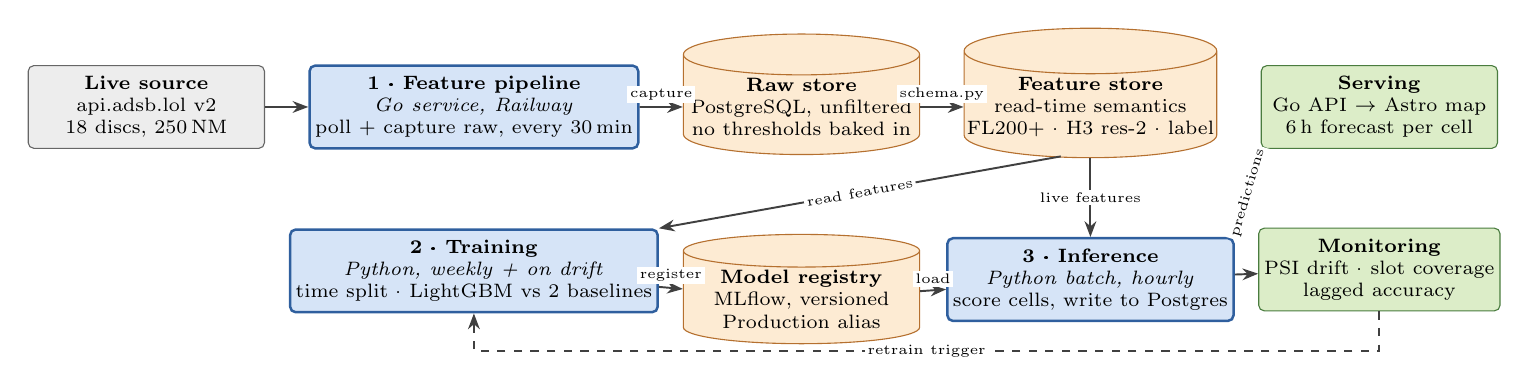
\begin{tikzpicture}[node distance=0.55cm and 0.55cm]
    % Row 1: capture and storage
    \node[src]   (src)  {\textbf{Live source}\\api.adsb.lol v2\\18 discs, 250\,NM};
    \node[pipe,  right=of src]  (feat) {\textbf{1 · Feature pipeline}\\\emph{Go service, Railway}\\poll + capture raw, every 30\,min};
    \node[store, right=of feat] (raw)  {\textbf{Raw store}\\PostgreSQL, unfiltered\\no thresholds baked in};
    \node[store, right=of raw]  (fs)   {\textbf{Feature store}\\read-time semantics\\FL200+ · H3 res-2 · label};
    \node[sink,   right=of fs]   (ui)   {\textbf{Serving}\\Go API $\rightarrow$ Astro map\\6\,h forecast per cell};
    % Row 2: training, registry, inference, monitoring
    \node[pipe,  below=1.0cm of feat] (train) {\textbf{2 · Training}\\\emph{Python, weekly + on drift}\\time split · LightGBM vs 2 baselines};
    \node[store, below=1.0cm of raw]  (reg)   {\textbf{Model registry}\\MLflow, versioned\\Production alias};
    \node[pipe,  below=1.0cm of fs]   (inf)   {\textbf{3 · Inference}\\\emph{Python batch, hourly}\\score cells, write to Postgres};
    \node[sink,   below=1.0cm of ui]   (mon)   {\textbf{Monitoring}\\PSI drift · slot coverage\\lagged accuracy};

    \draw[flow] (src) -- (feat);
    \draw[flow] (feat) -- node[lbl,above=1pt]{capture} (raw);
    \draw[flow] (raw) -- node[lbl,above=1pt]{schema.py} (fs);
    \draw[flow] (fs.south west) ++(0.25,0) -- node[lbl,sloped]{read features} (train.north east);
    \draw[flow] (train) -- node[lbl,above=1pt]{register} (reg);
    \draw[flow] (reg) -- node[lbl,above=1pt]{load} (inf);
    \draw[flow] (fs) -- node[lbl]{live features} (inf);
    \draw[flow] (inf.north east) -- node[lbl,sloped]{predictions} (ui.south west);
    \draw[flow] (inf) -- (mon);
    \draw[flow, dashed] (mon.south) -- ++(0,-0.5) -| node[lbl,pos=0.25]{retrain trigger} (train.south);
  \end{tikzpicture}
  \caption{FTI architecture. Blue: the three pipelines; orange: stores; solid arrows: data flow; dashed: retrain trigger.
           Deployed today: the live source, feature pipeline and raw store.}
\end{figure}
\vspace{-1.5ex}

\textbf{Pipelines and triggers.} (1)~\emph{Feature}: a Go service on Railway sweeps the 18
discs every 30 minutes and writes \textbf{unfiltered} observations to PostgreSQL: raw
coordinates, nullable altitude, no H3 cell and no label. Thresholds are applied at
\emph{read} time, so the altitude floor or H3 resolution can change and the whole history be
rebuilt. (2)~\emph{Training} (Python): weekly and on drift; reads the store, splits
chronologically, trains LightGBM against both baselines, logs to MLflow, registers the best
run. (3)~\emph{Inference} (Python): an hourly batch job, run after each sweep, that loads the
Production model and writes a 6-hour forecast per cell to a PostgreSQL table. A Go API serves
that table to an Astro frontend, so the request path never touches Python.

\textbf{Tech stack}, one line of rationale each:
\begin{itemize}
  \item \textbf{Languages:} Go wherever a process runs continuously in production (capture,
        serving API); Python only where the ML ecosystem is (features, LightGBM, MLflow).
  \item \textbf{Cloud and feature store:} Railway (container hosting) + PostgreSQL. Durable,
        unlike the 90-day CI artifacts it replaced, and SQL applies thresholds at read time.
  \item \textbf{Orchestration:} a long-lived Go service with a wall-clock ticker. Four
        staggered GitHub Actions crons captured only 53\,\% of hours over 74\,h (GitHub
        drops scheduled triggers and never retries), and here a missed hour is lost forever.
  \item \textbf{Tracking and registry:} MLflow, for run comparison and a Production alias
        that inference loads, so the deployed version is always identifiable.
  \item \textbf{Serving:} a Go JSON API plus an Astro frontend with an H3 map, both on
        Railway; static-first pages with a map island, and a map is the natural view of a
        spatial forecast.
  \item \textbf{Packaging and CI:} Docker, \code{uv.lock} for Python, Go modules; GitHub
        Actions runs lint and 50 tests (34 Python, 16 Go) against a real PostgreSQL.
\end{itemize}

\textbf{Training-serving skew} is prevented structurally: thresholds, altitude floor,
H3 resolution and lag set live once in \code{src/skyjam/common/schema.py} and are applied on
read. The Go capture service computes \textbf{no} label, and the sampling grid it shares with
Python has a parity test that fails the build if the two drift.

\textbf{Optional / stretch (not core):} Terraform IaC, Airflow, a managed feature store,
alerting on the drift metric. Core FTI comes first.

\textbf{Current state and risks.} The capture service is deployed and has completed 18/18
discs on every recent sweep. Risks: history accrues only from now on (mitigated by capturing
since proposal time and storing raw, so a definition change does not invalidate it); the API
could throttle or disappear (measured pacing, backoff, \code{adsb.fi} fallback); sparse night
traffic (per-cell traffic floor, unobserved cells excluded). \textbf{The repository is public:}
\url{\repo}.

\end{document}
